\documentclass{article}

\usepackage{polski}
\usepackage[utf8]{inputenc}
\usepackage{graphicx}
\usepackage{xcolor}
\usepackage{float}
\usepackage{caption}
\usepackage{array}
\usepackage{pbox}
\usepackage{tikz}
\usetikzlibrary{arrows}
\usepackage{amsmath}

\newcommand\tab[1][1cm]{\hspace*{#1}}

\title{Dokumentacja projektowa}
\date{2018-03-18}
\author{Jędrzej Kozal}

\begin{document}

\begin{titlepage}
	\centering
	
\includegraphics[width=0.25\textwidth]{logo_pol_wroclaw.png}\par\vspace{1cm}
	{\scshape\LARGE Politechnika Wrocławska \par}
	\vspace{1cm}
	{\scshape\Large Miekkie metody obliczeniowe\par}
	\vspace{1.5cm}
	{\huge\bfseries Zastosowanie Sieci Bayesa do diagnozowania ostrych stanów zapalnych \par}
	\vspace{2cm}
	{\Large\itshape Filip Guzy\par}
	{\Large\itshape Jędrzej Kozal\par}
	{\Large\itshape Michał Leś\par}

	\vfill
	prowadzący\par
	Mgr inż.~Mariusz \textsc{Kozioł}

	\vfill

% Bottom of the page
	{\large \today\par}
\end{titlepage}

\tableofcontents
\newpage


\section{Wstęp}

Celem projektu jest zbadanie skuteczności Sieci Bayesa w automatycznej diagnozie. Sieci Bayesa dobrze sprawują się dla zbilansowanych zbiorów zawierających zmienne dyskretne o znanych rozkładach, bądź zmienne dyskretne dla których możliwa jest estymacja parametryczna i nieparametryczna \cite{paper}. Zbiorem, który spełnia te wymagania jest Acute Inflammations Data Set dostępny w bazie UCI. Określając zagadnienie diagnozowania jako problem klasyfikacji można zmierzyć dokładność uzyskanego modelu. Osiągnięta dokładność dla sieci QMR została wyznaczona zgodnie z przyjętą metodyką.

\subsection{Wymagania projektowe}
W ramach projektu przewiduje się realizację poniższych podpunktów:
\begin{enumerate}
	\item Analiza danych wejściowych
	\item Przygotowanie danych wejściowych - dychotomizacja, dyskretyzacja
	\item Podział danych wejściowych umożliwiający ocenę klasyfikatora - projekt eksperymentu
	\item Wyznaczenie parametrów analizowanego zbioru potrzebnych do skonstruowania modelu (określenie prawdopodobieństw a priori i wspólnych rozkładów prawdopodobieństwa)
	\item Przygotowanie modelu - Sieci Bayesa w konfiguracji QMR - wyznaczenie topologii sieci
	\item Weryfikacja skuteczności modelu oraz analiza uzyskanych wyników
	\item Weryfikacja odporności modelu na wektory z brakującymi danymi
\end{enumerate}

Zakłada się, że uzyskany klasyfikator nie będzie klasyfikatorem słabym (klasyfikatory słabe osiągają dokładność zbliżoną do losowego wyboru klasy). Ze względu na brak wiedzy eksperckiej w omawianej dziedzinie, parametry modelu będą określane na podstawie zbioru uczącego. W efekcie powodzenie projektu będzie ściśle powiązane z jakością wykorzystanego zbioru danych. Innymi czynnikami, które mają wpływ na wynik eksperymentu są wiedza i umiejętności eksperymentatora.

\subsection{Wykorzystane narzędzia}
Do realizacji zadania wykorzystano środowisko Matlab, wraz z toolboxem BayesNet. Jest to darmowe narzędzie, dostępne do zanstalowania w środowisku Matlab. 

\section{Podstawy teoretyczne}
W tej sekcji zostaną omówione teoretyczne aspekty problemu oraz przyjętych rozwiązań.

\subsection{Omówienie zagadanienia}
W poniżej sekcji przedstawiono medyczne aspekty omawianego problemu.

\subsubsection{Zbiór uczący}
Jako zbiór danych uczących wykorzystano zbiór Acute Inflammations Data Set dostępny w bazie UCI \cite{data set}. Zawiera 120 próbek w większości binarnych lub dyskrenych. Autorzy uworzyli go z myślą o wspieraniu systemu ekspertowego, umożliwiającego diagnozę dwóch chorób układu moczowego - ostrego zapalenia pęcherza moczowego oraz odmiedniczkowego zapalenia nerek. Poniższe charakterystyki chorób zostały zaczerpnięte z opisu zbioru.

\paragraph{Ostre zapalenie pęcherza moczowego}
"Acute inflammation of urinary bladder is
characterised by sudden occurrence of pains in the abdomen region and 
the urination in form of constant urine pushing, micturition pains and 
sometimes lack of urine keeping. Temperature of the body is rising, 
however most often not above 38C. The excreted urine is turbid and 
sometimes bloody. At proper treatment, symptoms decay usually within 
several days. However, there is inclination to returns. At persons with 
acute inflammation of urinary bladder, we should expect that the illness 
will turn into protracted form."

\paragraph{Odmiedniczkowe zapalenie nerek}
"Acute nephritis of renal pelvis origin occurs considerably more often at 
women than at men. It begins with sudden fever, which reaches, and 
sometimes exceeds 40C. The fever is accompanied by shivers and one- or 
both-side lumbar pains, which are sometimes very strong. Symptoms of 
acute inflammation of urinary bladder appear very often. Quite not 
infrequently there are nausea and vomiting and spread pains of whole 
abdomen."

\subsubsection{Lista cech dostępnych w zbiorze uczącym}

W omawianym zbiorze dla każdego pacjenta znajdują się następujące parametry:

\begin{enumerate}
	\item Temperatura pacjenta 35C-42C
	\item Występowanie of nudności tak, nie
	\item Ból lędźwiowy tak, nie
	\item Urine pushing (nieustająca potrzeba oddawania moczu) tak, nie
	\item Ból w trakcie oddawania moczu tak, nie
	\item Pieczenie cewki moczowej, swędzenie, obrzęk ujścia cewki moczowej tak, nie
	\item decyzja: Zapalenie pęcherza moczowego tak, nie
	\item decyzja: Odmiedniczkowe zapalenie nerek tak, nie
\end{enumerate}


\subsection{Sieci Bayesa}

\subsubsection{Modelowanie probabilitystyczne}
W przypadku modelowania zależności między zmiennymi losowymi stosuje się wspólny rozkład prawdopodobieństwa (joint probabilty distribution, jpd). Dla dyskretnych zmiennych losowych stanowi ono tabelę z wszystkimi możliwymi kombinacjami wartości zmiennych. Dla 4 binarnych zmiennych losowych $A, B, C, D$ istnieje $2^4-1 = 15$ elementów tabeli. W ogólności liczba prawdopodobieństw $n$ zmiennych losowych w tabeli wynosi: $2^n - 1$. Funkcje wykładnicze bardzo szybko osiągają duże wartości, przez co modelowanie dla dużego $n$, może stanowić wyzwanie przez dużą liczbę paramterów.

\subsubsection{Definicja sieci Bayesa}
Sieć Bayesa to klasa modeli graficznych, w których do modelowania zależności między zmiennymi losowymi wykorzystuje się acykliczny graf skierowany. Wierzchołki grafu zawierają zmienne losowe, a krawędzie modelują zależności między zmiennymi losowymi. Wierzchołki połączone z wybranym wierzchołkiem przez krawedź wchodzącą nazywamy rodzicami (parent). Wierzchołki połączone przez krawędź wychodzącą nazywamy dziećmi (child). Wierzchołek nie posiadający rodziców nazywany jest korzeniem (root). Krawędzie grafu i jego struktura modelują zależności między zmiennymi losowymi, co pozwala na ogarniczenie ilości parametrów modelu.

\begin{figure}
\centering
	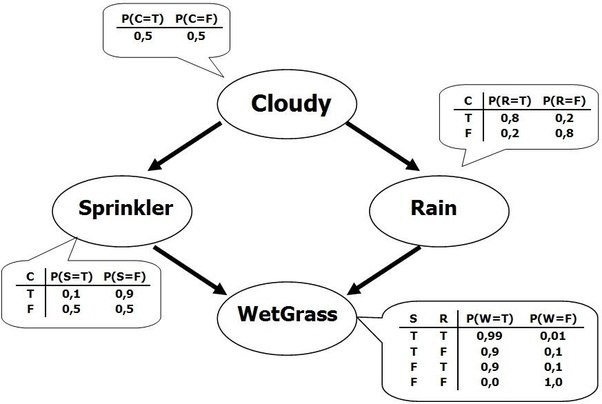
\includegraphics[width=0.80\textwidth]{net.jpeg}\par\vspace{1cm}
\caption{Przykładowa sieć Bayesa, modelująca wilgotność trawy, wraz z lokalnymi wspólnymi rozkładami prawdopodobieństwa. \\ źródło: https://towardsdatascience.com/introduction-to-bayesian-networks-81031eeed94e}
	\label{fig:net}
\end{figure}

Sieć Bayesa wykorzystuje założenie o niezależności zmiennych losowych do obliczania prawdopodobieństwa zmiennych losowych w wezłach, korzystając z prawdopodobieństwa wystąpienia konretnych wartości rodziców. 

Stosując regułę łańcucha dla prawdopodobieństwa, można zapisać wspólny rozkład prawdopodobieństwa jako:

\begin{equation}
	P(A, B, C, D) = P(A|B, C, D)P(B|C, D)P(C|D)P(D)
\end{equation}

Stosując założenie o niezależności $B$ od $C$ i $C$ od $D$ można tą samą regułę uprościć:

\begin{equation}
	P(A, B, C, D) = P(A|B, C, D)P(B|D)P(C)P(D)
\end{equation}

W ogólności dla Sieci Bayesa można zapisać:

\begin{equation}
	P(X_1, ... , X_n) = \prod_{i=1}^{n} P(X_i|Parents(X_i))
\end{equation}

Powoduje to znaczącą redukcję liczby parametrów modelu.

Przykładowa sieć Bayesa wraz z lokalnymi rozkładami prawdopodobieństwa została przedstawiona na rys. \ref{fig:net}. Poprzez podział tabel ze wspólnym rozkładem prawdopodobieństwa na mniejsze ilość paramterów modelu uległa zmianie z 15 do 18. Przy rosnącej ilości parametrów sieci Bayesa mogą przyczynić się do znaczącej redukcji liczby parametrów.

\subsubsection{D-separacja}

Pojęcie D-separacji może zostać wykorzystane do modelowania niezależności danych uczących ze zbioru. Jest ono ściśle powiązane ze strukturą sieci i opiera się na kilku zasadach. Przyjmijmy, że analizujemy dwie zmienne $X$ i $Y$. Zmienna losowa $Z$ znajduje się na ściężce $p$ w grafie między $X$ a $Y$.
\begin{enumerate}
\item Kiedy zmienna losowa $Z$ jest zdarzeniem warunkującym obliczanego prawdopodobieństwa (stanowi dowód, evidence) mówimy, że:
\begin{itemize}
 \item $Z$ jest zablokowane, jeżeli $p$ wchodzi do $Z$ od jego dziecka.
 \item $Z$ jest zablokowane, jeżeli $p$ wchodzi do $Z$ od jego rodzica i wychodzi od jego dziecka.
 \item $Z$ nie jest zablokowane, jeżeli $p$ wchodzi do $Z$ od jego rodzica wychodzi od jego rodzica.
\end{itemize}
\item Kiedy zmienna losowa $Z$ nie jest zdarzeniem warunkującym obliczanego prawdopodobieństwa mówimy, że:
\begin{itemize}
 \item $Z$ nie jest zablokowane, jeżeli $p$ wchodzi do $Z$ od jego dziecka.
 \item $Z$ nie jest zablokowane, jeżeli $p$ wchodzi do $Z$ od jego rodzica i wychodzi od jego dziecka.
 \item $Z$ jest zablokowane, jeżeli $p$ wchodzi do $Z$ od jego rodzica wychodzi od jego rodzica.
\end{itemize}
\end{enumerate}

$X$ jest niezależne od $Y$, jeżeli wszystkie możliwe ścieżki między $X$ a $Y$ w grafie są zablokowane.

$Z$ d-separuje $X$ od $Y$ (zapisywane: $X \perp_G Y|Z$), jeżeli wszystkie ścieżki między $X$ a $Y$ są zablokowane przez $Z$.

\subsubsection{Detekcja topologi sieci na podstawie danych uczących}

Ze względu na brak wiedzy dziedzinowej z zakresu medycyny, oraz braku możliwości konsultacji z ekspertem postanowiono wykorzystać metody pozwalające na nauczenie struktury sieci na podstawie zbioru uczącego.

W \cite{PhD} podano metody uczenia struktury sieci Bayesa. Wyróżna się dwie główne metody. Pierwsza z nich opiera się na maksymalizacji funkcji celu z wykorzystaniem maximum likelihood. Zaproponowano podejście w którym topologia sieci jest modyfikowana zgodnie z kierunkiem wzrostu maximum likelihood (hill climbing).

Drugą metodą opiera się na określeniu topologi na podstawie niezależności zmiennych losowych zbioru uczącego. Skierowany graf acykliczny jest nazywany I-mapą, jeśli:

\begin{equation}
	\forall_{X, Y, Z} (X \perp_G Y| Z) 	\Rightarrow  (X \perp_P Y | Z)
\end{equation}

Korzystając z zależności logicznej:

\begin{equation}
	p \Rightarrow q \Leftrightarrow \neg q \Rightarrow \neg p
\end{equation}

Aplikując poważyszy wzór dla sieci Bayesa można określić, że jeśli w domenowej dystrybucji P zmienne nie są niezależne to również nie powinny być niezależne w grafie (nie są d-separowane). W \cite{PhD} przedstawiono dokładny algorytm określania topologii sieci.

\subsubsection{Węzły Noisy OR}

Węzły Noisy OR w Sieciach Bayesa są probabilstycznym odpowiednikiem operacji logicznej OR. Dla dyskretnych węzłów $A, B$ i $C$ (gdzie $A$ i $B$ są przodkami $C$) definiuje się tablę prawdopodobieństw:

\begin{figure}[H]
\centering
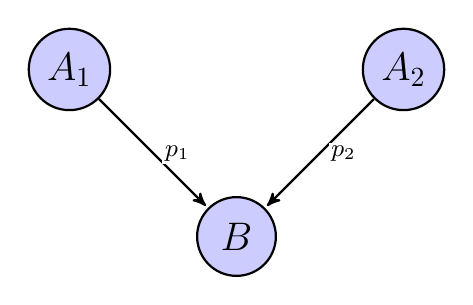
\begin{tikzpicture}[->,>=stealth',shorten >=1pt,auto,node distance=3cm,
  thick,main node/.style={circle,fill=blue!20,draw,
  font=\sffamily\Large\bfseries,minimum size=10mm}]

  \node[main node] (Aone) {$A_1$};
  \node[main node] (B) [below right of=Aone] {$B$};
  \node[main node] (Atwo) [above right of=B] {$A_2$};

  \path[every node/.style={font=\sffamily\small,
  		fill=white,inner sep=1pt}]
    (Aone) edge node[right=1mm] {$p_{1}$} (B)
    (Atwo) edge node[right=1mm]  {$p_{2}$} (B);
\end{tikzpicture}
\caption{Przykładowy schemat węzła noisy OR dla dwóch węzłów będących przodkami.}
\end{figure}

\begin{table}
\caption{Tabela prawdopodobieństw dla węzła nosiy OR}
\label{nosiy OR}
\centering
\begin{tabular}{|r|c|c|c|}
  \hline 
  $A_1$ & $A_2$ & P(B=F) & P(B=T)\\
  \hline
  F & F & $1$ & $0$\\
  \hline
  T & F & $p_1$ & $1-p_1$ \\
  \hline
  F & T & $p_2$ & $1-p_2$ \\
  \hline
  T & T & $p_1 p_2$ & $1 - p_1 p_2$ \\
  \hline
\end{tabular}
\end{table} 

Gdzie $p_A$ i $p_B$ są zdefiniowane jako prawdopodobieństwa hamowania dla węzłów $A$ i $B$. Można więc z łatwością zauważyć, że nawet gdy wszystkie wartości rodziców są równe T, to istnieje tylko co najwyżej prawdopodobieństwo, że wartość $C$ osiągnie T. Przyjmując $m$ rodziców analizowanego węzła możemy zapisać:

\begin{equation}
\begin{aligned}
	P(B|\mathbf{A}) &= 1 - P(\neg B | \mathbf{A}=T) \\
	&= 1 - \prod_{A_i \in \mathbf{A}=T} P(\neg B | A_i) \\
	&= 1 - \prod_{A_i \in \mathbf{A}=T} (1 - P(B|A_i)) \\
	&= 1 - \prod_{A_i \in \mathbf{A}=T} (1 - p_i)
\end{aligned}
\end{equation}

W trakcie obliczania prawodpodobieństwa aposteriori zdarzenia z węzła potomnego brane są pod uwagę tylko zdarzenia rodziców z wartością T. Prawdopodobieństwa mogą zostać wyestymowane na podstawie zbioru uczącego. Na podstawie powyższego równania można zapisać:

\begin{equation}
\begin{aligned}
	p_i = P(B|A_i) = \frac{P(A_i, B)}{P(A_i)}
\end{aligned}
\end{equation}

Gdzie $P(A_i, B)$ jest wspólnym rozkładem prawdopodobieństwa zmarginalizowanym tak, żeby zawierał tylko zmienne $A_i$ i $B$.

\subsubsection{Sieci QMR}

Sieci QMR są konfiguracją sieci często wykorzystywaną do przeprowadzania diagnostyki. W pierwszym rzędzie sieci występują potencjalne powody pewnych obserwowanych wielkości. W drugim rzędzie występują obserwowane wielkości. Wszystkie obserwowane wielkości są połączone z powodami przez węzły nosiy OR. Uczenie sieci QMR jest bardzo uproszczone.

\begin{figure}[H]
\centering
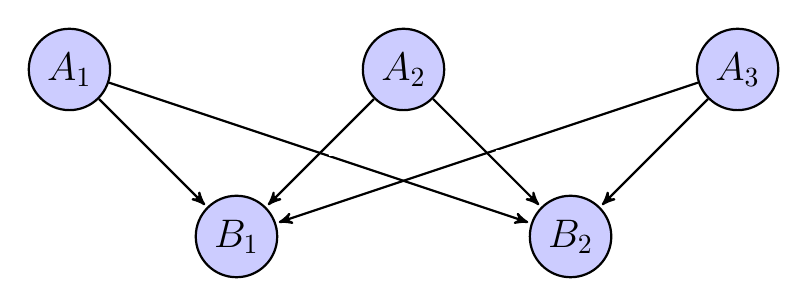
\begin{tikzpicture}[->,>=stealth',shorten >=1pt,auto,node distance=3cm,
  thick,main node/.style={circle,fill=blue!20,draw,
  font=\sffamily\Large\bfseries,minimum size=10mm}]

  \node[main node] (Aone) {$A_1$};
  \node[main node] (Bone) [below right of=Aone] {$B_1$};
  \node[main node] (Atwo) [above right of=Bone] {$A_2$};
  \node[main node] (Btwo) [below right of=Atwo] {$B_2$};
  \node[main node] (Athree) [above right of=Btwo] {$A_3$};

  \path[every node/.style={font=\sffamily\small,
  		fill=white,inner sep=1pt}]
    (Aone) edge node[right=1mm] {$$} (Bone)
    (Aone) edge node[right=1mm] {$$} (Btwo)
    (Atwo) edge node[right=1mm]  {$$} (Bone)
    (Atwo) edge node[right=1mm]  {$$} (Btwo)
    (Athree) edge node[right=1mm] {$$} (Bone)
    (Athree) edge node[right=1mm] {$$} (Btwo);
\end{tikzpicture}
\caption{Przykładowa Sieć QMR.}
\end{figure}

\section{Wykonane eksperymenty}

\subsection{Analiza danych wejściowych}

Zbiór zawiera 120 próbek. Dane są zbalansowane - dla obu zmiennych decyzyjnych występuje po odpowiednio 61 i 59 oraz 70 i 50 próbek należących do obu klas (zdrowy, chory). Wyklucza to konieczność stosowania oversamplingu lub undersamplingu. Poniżej omówiono sposób reprezentacji danych w przyjętym modelu.

\subsubsection{Dychotomizacja}
Dla każdej próbki wektor cech zawiera jedną cechę, która nie jest binarna. Istnieje wiele metod dyskretyzacji danych. Wiele z nich opiera się na wykorzystaniu średniej, wariancji i kwartyli zmiennych losowych. W przypadku projektu, przyjęto odmienne podejście. Korzystając z powszechnej wiedzy odnośnie występowania stanu podgorączkowego od 37.1 $^{\circ}$C zdychotomizowano temperaturę do stanów normalna i podwyższona. To rozwiązanie nie wymaga estymat obliczania momentów rozkładu, przez co jest bardziej odporne na zawartość zbioru uczącego. Po dychotomizacji każdy elemenet wektora w próbce ma wartość dyskretną, co znacząco ułatwia pracę z modelem.

\subsubsection{Reprezentacja wartości logicznych}
Przyjęto reprezentację wartości logicznych: 1 - false, 2 - true. Jest to wymaganie narzucone przez twórców toolboxa i prawdopodobnie jest związane z indeksowaniem maceirzy w matlabie od 1. 

\subsection{Projekt eksperymentu}
W nimniejszym rozdziale przedstawiono przyjęty sposob oceniania osiąganych wyników klasyfikatora

\subsubsection{Podział zbioru uczącego}
Cross validation. 20 i 100 próbek

\subsubsection{Przyjęte kryterium oceny klasyfikatora}
Definicja dokładności na podstawie tabeli pomyłek.

\begin{table}
\caption{Tabela pomyłek}
\label{nosiy OR}
\centering
\begin{tabular}{|r|c|c|c|}
  \hline 
  $A_1$ & Prawdziwa klasa P &Prawdziwa klasa N \\
  \hline
  Przewidziana klasa & TP & FP \\
  \hline
  Przewidziana klasa & FN & TN \\
  \hline
\end{tabular}
\end{table}

W tabeli pomyłek (confusion matrix) przedstawione są ilości próbke zaklasyfikowanych do wybranej kategori przez model w zależności od rzeczywistej klasy próbki. Na podstawie tabeli pomyłek można zdeafiniować najprostszą normę jakości klasyfikatora - dokładność. Dokładność jest zdefiniowana jako ilość poprawnie sklasyfikowanych próbek do wszystkich próbek ze zbioru uczącego.

\begin{equation}
	ACC = \frac{TP+TN}{TP+FP+TN+FN}
\end{equation}

W medycynie częściej stosowanymi normami dla testów są wskaźniki wiarygodności (Likelihood ratios) definiowane jako:

\begin{equation}
\begin{aligned}
	LR+ &= \frac{TPR}{FPR} = \frac{\frac{TP}{TP+FN}}{\frac{FP}{FP+TN}} \\ 
	LR- &= \frac{FNR}{TNR} = \frac{\frac{FN}{TP+FN}}{\frac{TN}{FP+TN}}
\end{aligned}
\end{equation}

$LR+$ opisuje stosunek częstości poprawnej klasyfikacji kalsy positive do częstości niepoprawnej klasyfikacji klasy negative. Im większa wartość $LR+$ tym większe prawdopodobieństwo występowania choroby.
$LR-$ opisuje stosunek częstości niepoprawnej klasyfikacji klasy positive do częstości poprawnej klasyfikacji klasy negative. Im mniejsza wartość $LR-$ tym większa braku choroby.

W projekcie przyjęto (...) jako normę do opisu jakości klasyfikatora.
Dla dwóch chorób ze zbioru uczącego wartości normy są obliczane niezależnie.
Dla zbioru uczącego i klasyfikatora losowego (przypisującego losową klasę nie zależnie od rzeczywistego stanu) wybrana norma przyjmuje wawrtości:

\begin{equation}
\begin{aligned}
  |choroba_1| = ? \\
  |choroba_2| = ?
\end{aligned}
\end{equation}


\section{Uzyskane rezultaty}

\newpage
\begin{thebibliography}{9}

\bibitem{data set}
J.Czerniak, H.Zarzycki, Application of rough sets in the presumptive diagnosis of urinary system diseases, 
Artifical Inteligence and Security in Computing Systems, ACS'2002 9th International Conference Proceedings, 
Kluwer Academic Publishers,2003, pp. 41-51 
\\\texttt{https://archive.ics.uci.edu/ml/datasets/Acute+Inflammations}

\bibitem{paper}
Ben-Gal I., Bayesian Networks, in Ruggeri F., Faltin F. \& Kenett R.,
Encyclopedia of Statistics in Quality \& Reliability, Wiley \& Sons (2007). 
\\\texttt{http://www.eng.tau.ac.il/~bengal/BN.pdf}

\bibitem{PhD}
Learning Bayesian Network Model Structure from Data, Dimitris Margaritis
May 2003, Carnegie Mellon University
\\\texttt{https://www.cs.cmu.edu/~dmarg/Papers/PhD-Thesis-Margaritis.pdf}

\bibitem{noisy OR}
Probabilistic Asthma Case Finding: A Noisy OR Reformulation
Vibha Anand, M.S., Stephen M. Downs, M.D., M.S.
AMIA Annu Symp Proc. 2008
\\\texttt{https://www.ncbi.nlm.nih.gov/pmc/articles/PMC2656011}

\bibitem{Towards Data Sience}
Introduction to Bayesian Networks, Towards Data Sience blog
\\\texttt{https://towardsdatascience.com/introduction-to-bayesian-networks-81031eeed94e}

\bibitem{bayesserver}
Baysian network software for Artificial Inteligence
\\\texttt{https://www.bayesserver.com/docs/introduction/bayesian-networks}

\end{thebibliography}
\newpage

\listoffigures
\newpage

\end{document}